\chapter{Full Interval Duty Cycle Manager}\label{sec:proposed_duty_cycle}
Figure \ref{fig:proposed_duty_cycle} explains how the proposed duty cycle manager enforces limits. It is simple to implement using a linked-list which gets culled whenever a tracked transmission falls outside the duty cycle interval. The method can quickly get complicated to visualise when dealing with more complex transmission scenarios  (e.g. short send, wait, short send, wait, long send, etc...). However, it is possible to identify when a transmission of a given length is allowed by searching ahead in time (e.g. using a binary search).
\begin{figure}[H]
    \centering
   	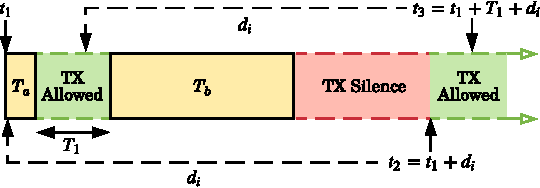
\includegraphics{Figures/duty_cycle_proposed}
    \caption[Proposed duty cycle enforcement method]{
    Proposed method for duty cycle limit enforcement. Behaviour can vary greatly depending on when transmissions occur and how long they are. This diagram is a partial representation and is valid provided there are no transmissions since $t=t_1-d_i$, where $d_i$ is the duty cycle interval (e.g. 3600 seconds). The duty cycle ($d_c$) shown is $\frac{T_a + T_b}{d_i}$. Enforcement is handled as follows. Immediately after the first transmission occurs, the remaining interval allowance is $T_b$ ($T_a+T_b-T_a$). For purposes of demonstration, a short period of silence occurs. Once the transmission of length $T_b$ occurs, the remaining interval allowance is 0 ($T_b - T_b$), therefore the transmitter must be silent until allowance is freed. At $t_2$ a transmission of length $T_a$ would be allowed because for every time unit of a new transmission, the corresponding time unit of $T_a$ would no longer fall in the time interval. A longer transmission would not be allowed until $t_3$ because $T_b$ will not fall outside of the time interval until $T_1$ has elapsed. Note that as $T_a$ is already available the transmission can start $T_a$ before $T_b$ actually falls out of the interval. Therefore at $t_3$ a transmission of $T_a + T_b$ would be allowed (in this case, the full interval limit). The figure is not to scale.    
    }
    \label{fig:proposed_duty_cycle}
\end{figure}

